% --- Knowledge distillation: motivation and teacher--student ---
\begin{frame}[plain]
  \centering
  \vfill
  {\LARGE\bfseries Model Optimisation Techniques}
  \vfill
\end{frame}

% Harvard AC215 L11 slides 8--10: distillation as a compression theme; deployment vs training; history
\begin{frame}{Distillation}
  \centering
  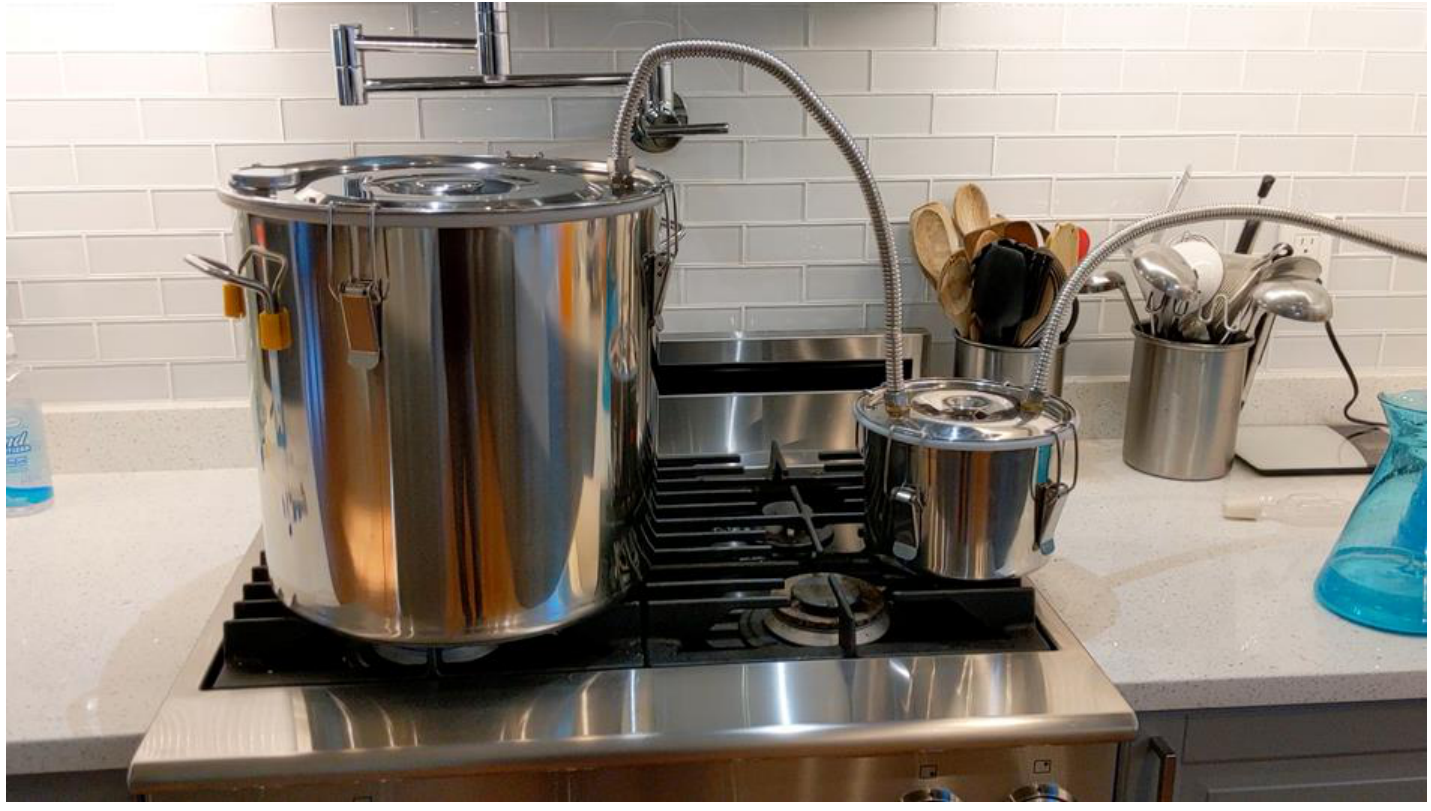
\includegraphics[width=\linewidth,height=0.9\textheight,keepaspectratio]{assets/New-Lecture-Inference_Optimisation/harvard_L11_compression_p08.png}\\[0.35em]
  {\scriptsize Harvard IACS AC215, Lecture 11 --- \href{https://harvard-iacs.github.io/2024-AC215/assets/lectures/lecture11/L11_compression_techniques.pdf}{Slides}.}
\end{frame}

\begin{frame}{Compression Technique: Distillation}
  \textbf{\textcolor{blue}{Problem:}}
  \begin{itemize}\itemsep0.45em
    \item During \href{https://en.wikipedia.org/wiki/Training,_machine_learning}{\textcolor{blue}{training}}, a model does not have to operate in real time and does not necessarily face restrictions on computational resources. The primary goal is to extract as much structure from the given data as possible.
    \item But latency and resource consumption do become of concern if the model is to be deployed for \href{https://en.wikipedia.org/wiki/Inference_(machine_learning)}{\textcolor{blue}{inference}}.
  \end{itemize}
  \vspace{0.6em}
  {\color{red}\textbf{So what?}}~We must develop ways to compress models for inference.
\end{frame}

\begin{frame}{Compression Technique: Distillation}
  \textbf{\textcolor{blue}{Idea:}}
  \begin{itemize}\itemsep0.45em
    \item In 2006, Bucil\u{a} et al.\ showed that it was possible to transfer knowledge from a large trained model (or ensemble of models) to a smaller model for deployment by \textcolor{blue}{\textbf{training it to mimic the larger model's output}}.
    \item In 2014 Hinton et al.\ generalized the process and gave the name \textcolor{blue}{\textbf{Distillation}}.
  \end{itemize}
  \vspace{0.5em}
  Main idea of distillation is that \textbf{\textcolor{red}{training and inference are 2 different tasks}};\newline
  thus a \textbf{\textcolor{red}{different model should be used}}.
\end{frame}

\begin{frame}{Distillation: Teacher -- Student}
  \textbf{\textcolor{red}{Assumption:}} If we can achieve similar convergence using a \textbf{smaller network}, then the convergence space of the Teacher Network should \textbf{overlap} with the solution space of the Student Network.
  \vspace{0.7em}
  \centering
  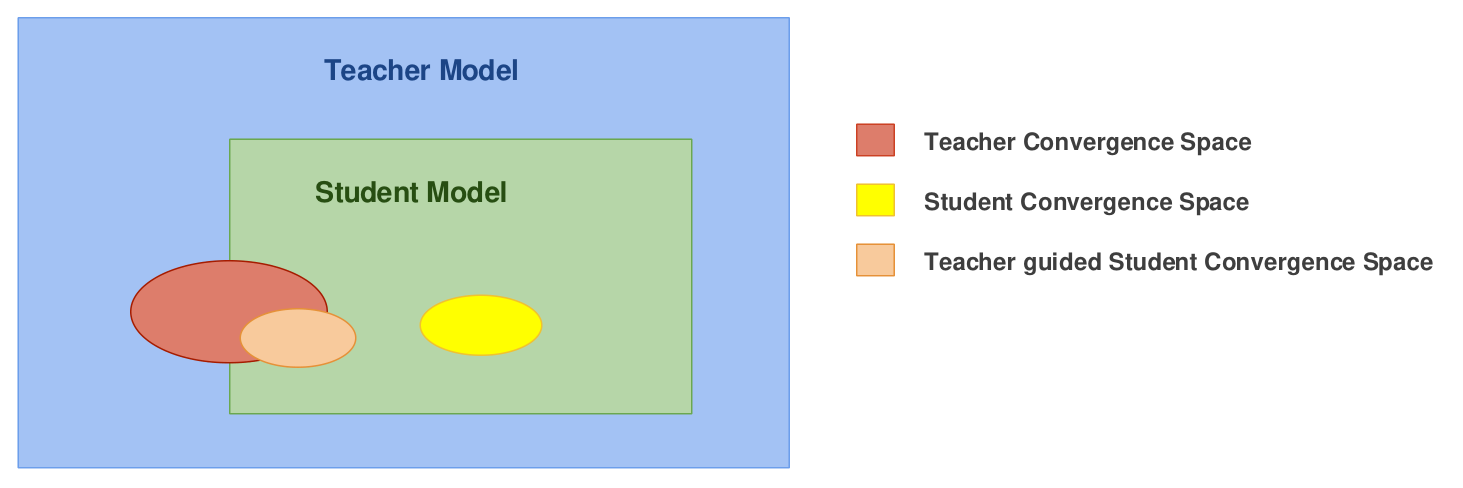
\includegraphics[width=0.9\linewidth,height=0.36\textheight,keepaspectratio]{assets/New-Lecture-Inference_Optimisation/harvard_L11_compression_p12.png}\\[-0.1em]
  {\scriptsize \textit{Teacher/Student convergence regions. Harvard AC215, L11.}}
\end{frame}

